\section{Project Guidelines}
\subsection{Deployment Plan}

\subsubsection{Gantt chart for project schedule}

    \begin{figure}[h]
        \centering
        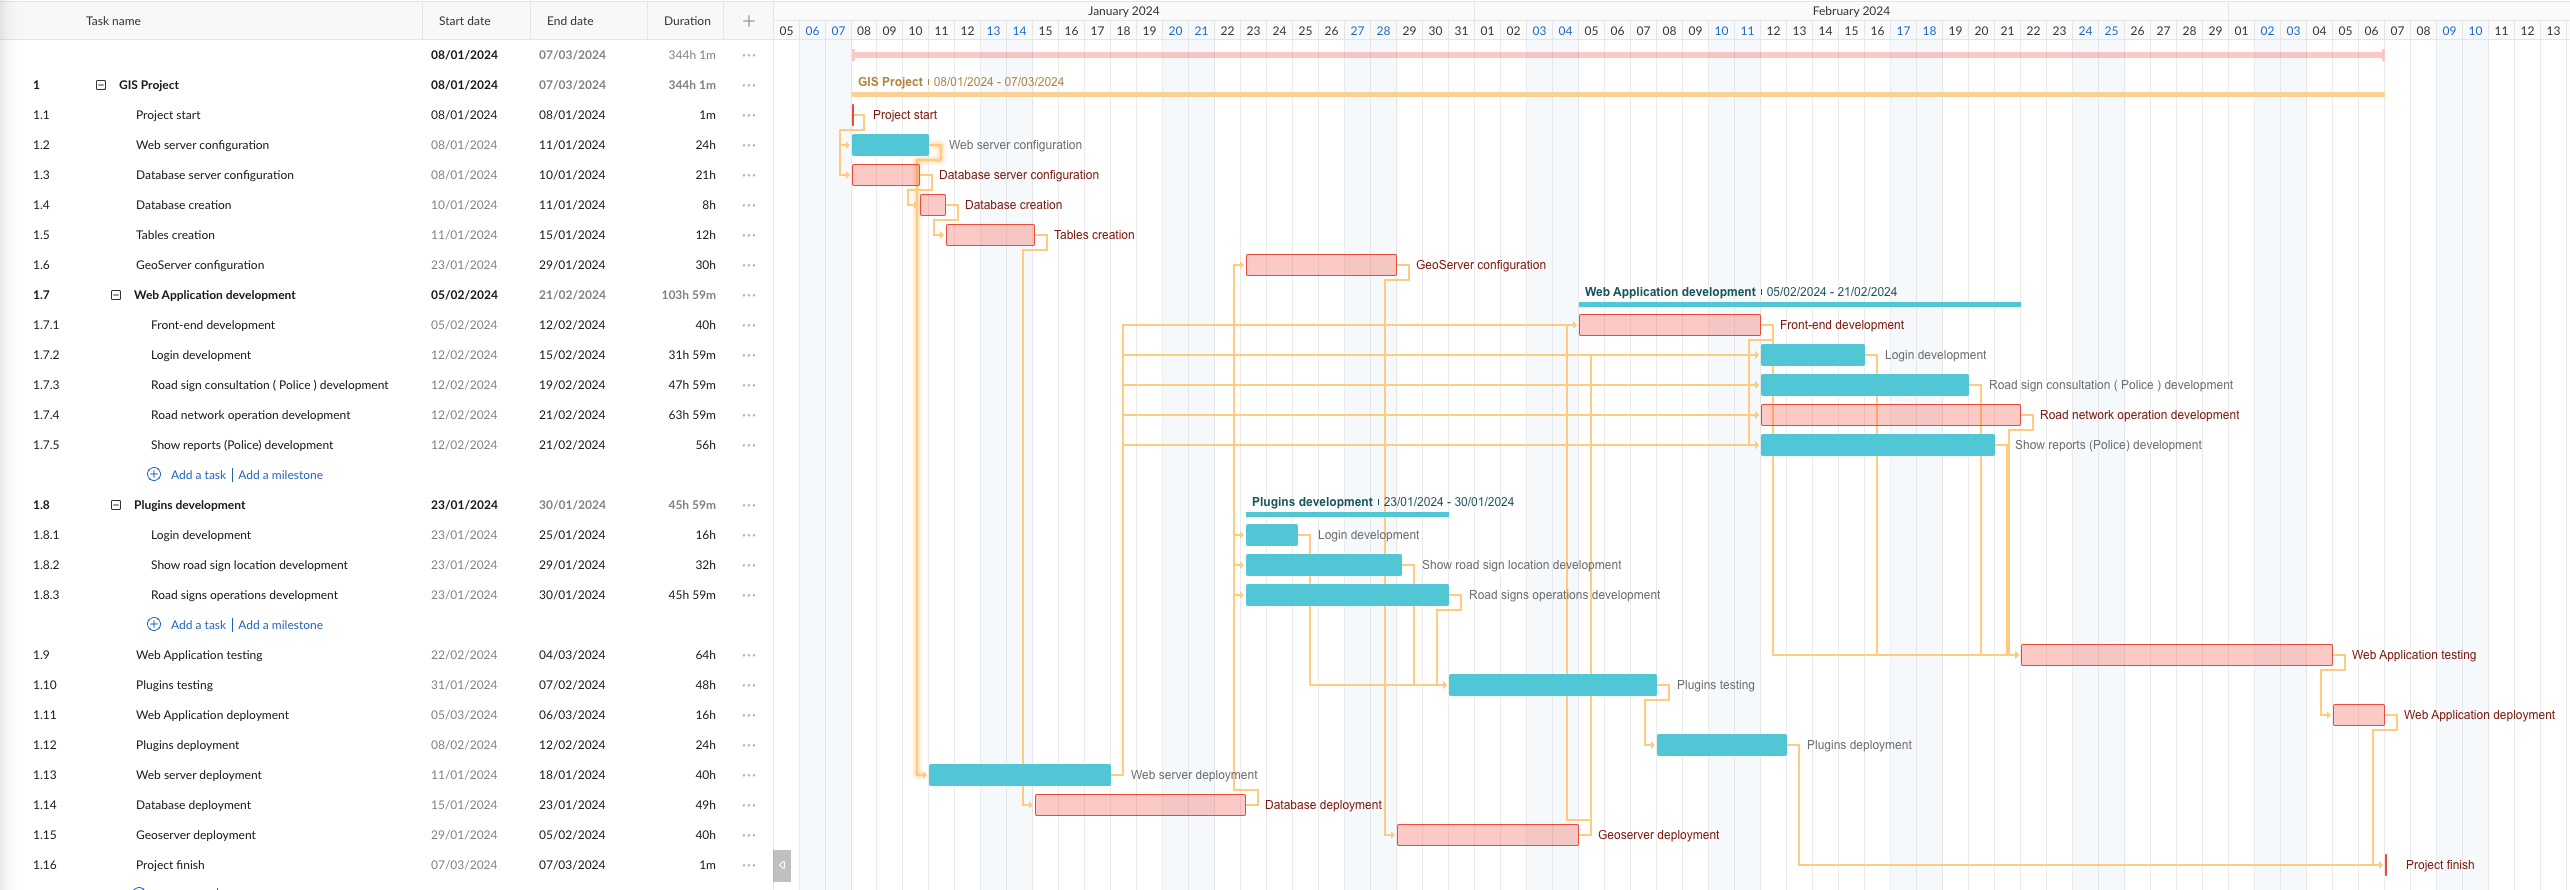
\includegraphics[width=0.7\textwidth]{images/GANTT.png}
        \caption{Gantt schema}
       \end{figure}

\subsubsection{Gantt description}
From the Gantt schema, it is possible to identify the critical path in red, which is the longest path from the start of the project to the end of it: this means that a delay of an activity belonging to the critical path produces a delay on the entire project.
The project starts with the Web Server configuration the 8/01/2024 and it should be finish without delay after the Web Application is fully deployed the 7/03/2024.
In the Gantt chart only activity are listed: the number of human resources which the project relies on are not present, since they are not known how many of them they will work.
After the possible project acceptance, the Gantt schema should be revisited adding how many people are available to work for the project.

\subsubsection{Milestones and Deliverables}
The project has two milestones, each one associated to a deliverable:
\begin{itemize}
    \item \textbf{Web Application development ended}: after the \textit{Show reports ( Police ) development} activity is ended the Web Application development is ended
    \item \textbf{openJUMP plugins development ended} after the \textit{Road sign operations development} activity is ended the plugins development is ended
\end{itemize}

\newpage

\subsection{Benefits Evaluation}
\subsubsection{Benefits Identification}
After a rigorous analysis of the system, we identify the following internal and external benefits.
\begin{itemize}
    \item \textbf{INTERNAL BENEFITS}
    \begin{enumerate}
        \item \textbf{Laws and standards conformity:} the system will follow the national and international standards, laws and guidelines for the management of road networks. In this way the province of Padova will be a promoter of innovation in road management with related signs and safety devices.
        \item \textbf{Reduction of operating costs:} thanks to the reports made by citizens and the plugins offered by the System, the office technicians will reduce the time to perform maintenance works since they will only have to follow the path calculated by the plugin and not go looking for road holes around the city.
        \item \textbf{Increasing of the efficiency and reputation:} the presence of the reports will allow a shorter time from the moment a hole is reported to the day when the technicians take action for the maintenance. All these things will lead to faster and more effective works, also improving the image of the city and road management office.
        \item \textbf{Re-engineering of the processes:} the adoption of new software and systems will allow for a general renewal in the management of the road network, enabling a new avenue for the use of technology in the management of public entities.
    \end{enumerate}
    \item \textbf{EXTERNAL BENEFITS}
    \begin{enumerate}
        \item \textbf{Improving citizen satisfaction:} by involving citizens in reporting problems with the road network, it can lead to an improvement in citizens' opinion of the city administration as well as in the city itself.
        \item \textbf{Improving citizen travels:} thanks to the web portal, citizens can check the areas with the greatest presence of road holes by avoiding going through those streets unless strictly necessity.
        \item \textbf{Reduction of risks:} by speeding up maintenance time, the system will enable citizens to travel on safer and more efficient roadways. This will reduce the risk of accidents caused by road holes or damaged traffic signals and safety devices.
    \end{enumerate}
\end{itemize}

\subsubsection{Economic Quantification of the Benefits}
Making an accurate economic estimate brought by the benefits described in the previous section is not easy. Despite the great importance of all the internal benefits that help in the economic and administrative management of the road network, we can say that the most important benefit brought by this project is the improvement of the quality in the experience that citizens have on a daily basis. \\ In fact, every day thousands of people move through the streets of Padova, whether on foot, bicycles, public transportations or automobiles. Surely meeting their needs by moving on safe and efficient streets is a huge benefit that the city can enjoy thanks to the street management offered by this System.\\
Some benefits that can be quantified instead are, for example:
\begin{itemize}
    \item \textbf{Laws and standard conformity:} the compliance with standards and laws will allow to integrate other new functionalities based on future available data. Moreover, this will allow the administration to sell data acquired from reports to other companies earning money to invest in the maintenance of the roads.
    \item \textbf{Reduction of operating costs:} thanks to the reports made by citizens, there will be a decrease in the intervention times of maintenance technicians, also reducing the number of technicians needed. This will lead to savings of a monthly salary of 1500 euros per technician.
\end{itemize}

\subsection{Risk Management}
Assessing and managing software project risks requires a comprehensive approach. It involves identifying and documenting risks, assessing their likelihood and impact, and developing mitigation strategies and contingency plans. Continuous communication and  monitoring, and the use of specialized tools are essential to release a final good product.


For the purpose of the above outlined project, it has been employed the Risk Matrix and the Risk Register as essential tools to evaluate and analyze the magnitude of risk associated with different aspects and components.

A noticeable part that is not present since is will take place with the project ongoing is the project failure;
Since the project is quite big, the possibility that everything goes as planned is low. \\
The key point is to reduce the failure during the project development, by setting a threshold on extra money, time, human resources that will be necessary to continue the project.
As conclusion is important to learn from the mistakes made, to improve or change the critical part of the project, using (if necessary) more resources to accomplish the goals defined.
\subsubsection{Risk Matrix}

\begin{table}[htbp]
    \centering
    \begin{tabular}{|cc|c|c|c|}
    \hline
    \multicolumn{2}{|l|}{\textbf{IMPACT}}                      & LOW    & MEDIUM & HIGH   \\ \hline
    \multicolumn{1}{|l|}{\multirow{3}{*}{\rotatebox{90}{\textbf{LIKE.}}}} & HIGH   & \cellcolor{MediumRiskColor}MEDIUM & \cellcolor{HighRiskColor}HIGH & \cellcolor{HighRiskColor}HIGH   \\ \cline{2-5} 
    \multicolumn{1}{|l|}{}                   & MEDIUM & \cellcolor{LowRiskColor}LOW    & \cellcolor{MediumRiskColor}MEDIUM & \cellcolor{HighRiskColor}HIGH   \\ \cline{2-5} 
    \multicolumn{1}{|l|}{}                   & LOW    & \cellcolor{LowRiskColor}LOW    & \cellcolor{LowRiskColor}LOW    & \cellcolor{MediumRiskColor}MEDIUM \\ \hline
    \end{tabular}
    \caption{Risk Matrix}
    \label{matrix}
\end{table}
\newpage
\subsubsection{Risk Register}    
\begin{table}[htbp]
    \centering
    \caption{Risk Register} 
    \small\resizebox{\textwidth}{!}{
    \begin{tabular}{|*{7}{>{\centering\arraybackslash}m{2.2cm}|}}  
        \hline
        \textbf{RISK INFO} & \textbf{CAUSE} & \textbf{DAMAGE} & \textbf{LIKELI- \allowbreak HOOD} & \textbf{IMPACT} & \textbf{SEVERITY} & \textbf{ACTION}\\ 
        \hline
        Data Breach & The potential attacker using SQL injections tries to steal sensitive information & Stealing of sensitive data & \cellcolor{MediumRiskColor}MEDIUM & \cellcolor{HighRiskColor} HIGH &  \cellcolor{HighRiskColor} HIGH & Mitigate \\ \hline
        Denial of Service & The attacker submits too many requests to the Web server in order to make it unavailable & System is not longer available to use & \cellcolor{LowRiskColor}LOW & \cellcolor{HighRiskColor}HIGH & \cellcolor{MediumRiskColor} MEDIUM & Transfer \\ \hline
        Man in the Middle & The potential attacker intercepts and potentially alters informations between the provincial office and the internal servers & Stealing of sensitive data and possible Industrial espionage & \cellcolor{LowRiskColor}LOW & \cellcolor{HighRiskColor}HIGH & \cellcolor{MediumRiskColor} MEDIUM & Mitigate \\ \hline
        Fake reports & User submits fake reports about non existing road damage & Not useful data present in the system & \cellcolor{MediumRiskColor} MEDIUM & \cellcolor{LowRiskColor}LOW & \cellcolor{LowRiskColor}LOW & Accept \\ \hline
    \end{tabular}}
\end{table}




\newpage
\subsection{Cost analysis}
In this section, they will be outlined the cost of developing GIS system previously described.
Into the making of a project, there are two types of cost: the cost of the project itself, plus costs that are needed to maintain and renew the system.


\subsubsection{Project cost}
In the table below, there are three types of costs:
\begin{itemize}
    \item \textbf{technician cost}: this € 20  unit cost is associated to one hour of work from an external technician to setup one of the three servers.
    \item \textbf{WebApp developer cost}: € 50 is the amount of money that the developer of the Web Application will receive for one hour of work.
    \item \textbf{Java developer cost}: € 35 is the amount of money that the developer of the openJUMP plugins will receive for one hour of work. 
\end{itemize}
It is important to say that the costs in Table 3 are just an estimate of the final cost of the project, that would be only possible to have after the end of the project.
\begin{table}[htbp]
    \centering
    \label{cost}
    \caption{Project Cost Breakdown} 
    \begin{tabular}{lrrr}
        \toprule
        Activity & Unit cost & Quantity & TOTAL \\
        \midrule
        Web Server configuration & 20 & 24h & €480,00 \\
        DB Server configuration & 20 & 21h & €420,00 \\
        Geo Server configuration & 20 & 30h & €600,00 \\
        DB creation & 20 & 8h & €160,00 \\
        Tables creation & 20 & 12h & €240,00 \\
        Webapp development & 50 & 240h & €12,000,00 \\
        Plugins development & 35 & 94h & €3,290,00 \\
        Webapp testing & 50 & 64h & €3,200,00 \\
        Plugins testing & 35 & 48h & €1680,00 \\
        Webapp deployment & 50 & 16h & €800,00 \\
        Plugin deployment & 35 & 8h & €280,00 \\
        Web Server deployment & 20 & 40h & €800,00 \\
        DB deployment & 20 & 49h & €980,00 \\
        Geo Server deployment & 20 & 40h & €800,00 \\
        \midrule
        TOTAL & & & €25,730,00 \\
        \bottomrule
    \end{tabular}
\end{table}

\newpage 

\subsubsection{Running costs}
In the running costs table, there two types of costs: the one regarding the Server maintenance that it is carried out once year and its fixed, and the cost associated to the assistance, which it depends on how many hours a year a technician on-site or remotely, will be necessary for troubleshooting.
\begin{table}[htbp]
    \centering
    \caption{Project Cost Breakdown} 
    \begin{tabular}{lrrr}
        \toprule
        Activity & Unit cost & Quantity & TOTAL \\
        \midrule
        Server maintenance & 1500 & 1 & €1500,00 \\
        Remote assistance & 20 & X & €20*X \\
        On-site assistance & 30 & X & €30*X \\
        \midrule
        TOTAL & & & €1500,00 + variable costs \\
        \bottomrule
    \end{tabular}
\end{table}